%%%%%%%%%%%%%%%%%%%%%%%%%%%%%%%%
%                              %
% Luther Michaels              % 
% ECE 351-52                   %
% Lab 6                        %
% October 14, 2021             %
% Partial Fraction Expansion   %
%                 Lab Report   %
%                              %
%%%%%%%%%%%%%%%%%%%%%%%%%%%%%%%%



%%%%%%%%%%%%%%%%%%%%%%%%%%%%%%%%%%%%%%%%%%%
%%% DOCUMENT PREAMBLE %%%
\documentclass[12pt]{report}
\usepackage[english]{babel}
\usepackage{url}
\usepackage[utf8x]{inputenc}
\usepackage{amsmath}
\usepackage{graphicx}
\graphicspath{{images/}}
\usepackage{parskip}
\usepackage{fancyhdr}
\usepackage{vmargin}
\usepackage{listings}
\usepackage{hyperref}
\usepackage{xcolor}

\newcommand{\adj}{\hspace{0.001em}}

\definecolor{codegreen}{rgb}{0,0.6,0}
\definecolor{codegray}{rgb}{0.5,0.5,0.5}
\definecolor{codeblue}{rgb}{0,0,0.95}
\definecolor{backcolour}{rgb}{0.95,0.95,0.92}

\lstdefinestyle{mystyle}{
	backgroundcolor=\color{backcolour},   
	commentstyle=\color{codegreen},
	keywordstyle=\color{codeblue},
	numberstyle=\tiny\color{codegray},
	stringstyle=\color{codegreen},
	basicstyle=\ttfamily\footnotesize,
	breakatwhitespace=false,         
	breaklines=true,                 
	captionpos=b,                    
	keepspaces=true,                 
	numbers=left,                    
	numbersep=5pt,                  
	showspaces=false,                
	showstringspaces=false,
	showtabs=false,                  
	tabsize=2
}

\lstset{style=mystyle}

\setmarginsrb{3 cm}{2.5 cm}{3 cm}{2.5 cm}{1 cm}{1.5 cm}{1 cm}{1.5 cm}

\title{6}	% Title						
\author{Luther Michaels}	% Author		
\date{October 14, 2021}   % Date

\makeatletter
\let\thetitle\@title
\let\theauthor\@author
\let\thedate\@date
\makeatother

\pagestyle{fancy}
\fancyhf{}
\rhead{\theauthor}
\lhead{\thetitle}
\cfoot{\thepage}
%%%%%%%%%%%%%%%%%%%%%%%%%%%%%%%%%%%%%%%%%%%%

\begin{document}
	
%%%%%%%%%%%%%%%%%%%%%%%%%%%%%%%%%%%%%%%%%%%%%%%%%%%%%%%%%%%%%%%%%%%%%%%%%%%%%%%%%%
%%% TITLE PAGE %%%
\begin{titlepage}
	\centering
	\vspace*{0.5 cm}
		
	\begin{center}    
		\textsc{\Large   ECE 351 - Section \#52}\\[2.0 cm]	
	\end{center}  
	\textsc{\Large Partial Fraction Expansion }\\[0.5 cm]
	\rule{\linewidth}{0.2 mm} \\[0.4 cm]
	{ \huge \bfseries \thetitle}\\
	\rule{\linewidth}{0.2 mm} \\[1.5 cm]
	\begin{minipage}{0.4\textwidth}
		\begin{flushleft} \large
		\end{flushleft}
	\end{minipage}~
	\begin{minipage}{0.4\textwidth}
		\begin{flushright} \large
			\emph{Submitted By:} \\
			Luther Michaels \break
				
			\emph{Submission Date:} \\
			October 14, 2021
		\end{flushright}
	\end{minipage}\\[2 cm]
\end{titlepage}
	
%%%%%%%%%%%%%%%%%%%%%%%%%%%%%%%%%%%%%%%%%%%%%%%%%%%%%%%%%%%%%%%%%%%%%%%%%%%%%%%%%%
%%% TABLE OF CONTENTS %%%
	
\tableofcontents
\pagebreak
	
%%%%%%%%%%%%%%%%%%%%%%%%%%%%%%%%%%%%%%%%%%%%%%%%%%%%%%%%%%%%%%%%%%%%%%%%%%%%%%%%%%
%%% LAB REPORT %%%
\renewcommand{\thesection}{\arabic{section}}
\section{Introduction}

The central focus in this lab is the concept of partial fraction expansion (PFE). The goal is to introduce and build familiarity with the scipy.signal.residue() Python package function. Python commands will be used to verify both a step response derived by hand using the PFE method and its associated residues, poles, and coefficients. A higher order differential can then be analyzed in Python, plotting its step response and verifying the result. \\

The step function created in an early lab will be utilized once again in this procedure. The central function of interest is scipy.signal.residue() which returns three arrays containing the elements of the partial fraction of its input. The numpy commands np.real and np.imag can be used to isolate only the real or imaginary parts of these outputs. The scipy.signal.step() function will also be useful to verify step responses. All functions and plots can be produced using proper hand derivation and implementation via Python code written within the Spyder software. \\
	
\section{Equations}

\begin{equation*}
	u(t)=
	\begin{cases}
		0 & t < 0 \\
		1 & t \ge 0 \\
	\end{cases}
\end{equation*}
\begin{equation}
	y_c(t) = 2|k|e^{-\alpha t}cos(\omega t + \!< \! k)u(t)
\end{equation}
\begin{equation*}
	y_1\adj'(t) + 10y_1\adj'(t) + 24y_1(t) = x''(t) + 6x'(t) + 12x(t)
\end{equation*}
\begin{equation}
	H_1(s) = \frac{Y_1(s)}{X(s)} = \frac{s^2 + 6s + 12}{s^2 + 10s + 24}
\end{equation}
\begin{align}
	Y_1(s) &= \frac{s^2 + 6s + 12}{s(s^2 + 10s + 24)} \\
	&= \frac{1}{2s} - \frac{1}{2(s + 4)} + \frac{1}{s + 6}
\end{align}
\begin{equation}
	y_1(t) = (\frac{1}{2} - \frac{1}{2}e^{-4t} + e^{-6t})u(t)
\end{equation}
\begin{equation*}
	y_2\adj^{(5)}(t) + 18y_2\adj^{(4)}(t) + 218y_2\adj^{(3)}(t) + 2036y_2\adj^{(2)}(t) + 9085y_2\adj^{(1)}(t) + 25250y_2(t) = 25250x(t)
\end{equation*}
\begin{equation}
	H_2(s) = \frac{Y_2(s)}{X(s)} = \frac{25250}{s^5 + 18s^4 + 218s^3 + 2036s^2 + 9085s + 25250}
\end{equation}
\begin{equation}
	Y_2(s) = \frac{25250}{s(s^5 + 18s^4 + 218s^3 + 2036s^2 + 9085s + 25250)}
\end{equation}
	
\section{Methodology}

The necessary transfer function and step response derivations for this lab were accomplished in the prelab and provided above as Equations 2 and 5 respectively. The first task of Part 1 in the lab manual requested that this step response be plotted between 0 and 2s using Python. Equation 5 was implemented as its own function of time using numpy.exp as needed. The step size was initialized to $ 1\times 10^{-5} $ for good resolution and the time interval was set with numpy.arange. The function was then graphed as the first subplot in a joint plot using the same sequence of commands in matplotlib.pyplot as in prior experiments. \\

Task 2 of Part 1 required the step response plot be verified using scipy.signal.step() on the transfer function in Equation 2. This was achieved by creating two equal-size matrices that held the coefficients of the numerator and denominator as aligned by their associated orders of magnitude. These matrices were used as inputs to the scipy function along with the time variable, and the output was plotted as the second subplot of the figure created in Task 1. \\

The third task of Part 1 involved verifying that the residues, poles, and coefficients found using Python matched those reflected in Equation 4. The numerator and denominator arrays assigned in the prior task were updated to include the step function input as shown in Equation 3. This necessitated that an extra 0 be included at the start of the numerator array and another at the end of the denominator. The scipy.signal.residue() function was then called using the two arrays and time variable, and the output arrays were collected in three variables. The results were printed to the console in order to enable a comparison. \\

Task 1 of Part 2 mirrored the procedure of Task 3 above. The higher order differential was represented in numerator and denominator arrays corresponding to Equation 7. This incorporated the step function as its input. The three resultant arrays of the scipy.signal.residue() function were printed for use in an upcoming task. \\

The second task of Part 2 requested that the time-domain step response of this differential be plotted between 0 and 4.5s using the results of the previous task. A function was created for this response by employing the obtained residues and poles in the general form dictated by the cosine method shown in Equation 1. As the PFE results were stored in arrays, a loop was created to iterate through the results at each index. The duration of iteration was determined using the len() command on one of the arrays. The equation was implemented using the package commands numpy.abs, numpy.angle, numpy.real, and numpy.imag on the residues and poles as prescribed. The multiplication by 2 in Equation 1 was not included; the residue was used for the variable k. The final step response was returned as the sum of the cosine method applied for each index. The time interval was set with numpy.arange and the plot was created. Limits on the y-axis were later imposed using matplotlib.pyplot.ylim() to match the results of the plot in the following task. \\

\begin{lstlisting}[language=Python]
""" PART 2, TASK 2: PLOT TIME-DOMAIN STEP RESPONSE """
def s_resp(t):
	y = 0  # summation initialization
	for i in range(len(R)):  # length of residue arrays
	y += (np.abs(R[i]) * np.exp(np.real(P[i]) * t) * np.cos((np.imag(P[i]) * t) + np.angle(R[i])) * u(t))
return y
\end{lstlisting}

In the third task of Part 2, the objective was to graphically verify the results of the step response plot in the prior task. The numerator and denominator arrays created in Task 1 of Part 2 were altered to represent the general transfer function shown in Equation 6. This meant that the initial 0 in the numerator array had to be removed along with the final 0 in the denominator. The scipy.signal.step() function was then called with the two arrays and time variable. The step output was plotted over the same time interval as the result of the cosine method to facilitate a comparison. \\

Github Link: \url{https://github.com/Luther-Michaels} \\
	
\section{Results}

The plots for the step response derived by hand calculation and using scipy.signal.step() are shown in the top and bottom subplots respectively of the below figure. The time interval is properly set between 0 and 2s as requested. Our expectation given by Equation 5 is supported by the shapes' general correspondence to an exponential decay. The initial y-axis value of the equation also corresponds to the step function at a time of zero, which would be the result of an evaluation with t = 0. Likewise, the final y-axis value of 0.5 aligns with the prescription the Final Value Theorem has for the end behavior. When s equals zero, Equation 2 simplifies to 0.5. The fact that both subplots obtained through alternate methods match completely is evidence of their accuracy.  The step size has been set to a small enough value that it provides sufficient resolution. \\
	
\begin{center}
	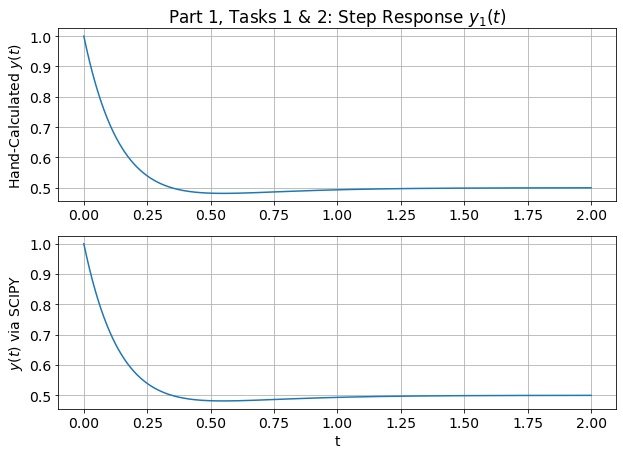
\includegraphics[scale = 0.6]{Lab 6 - Plots/Part1-Tasks1&2.png}\\[1.0 cm]
\end{center}

The printed results of the partial fraction expansion of Equation 3 using scipy.signal.residue() can be found in the Appendix. The values determined for the residues, poles, and coefficients are given in this order below:
\begin{align*}
	R &= [0.5\enspace -\!0.5\quad 1] \\
	P &= [0\enspace -\!4\enspace -\!6] \\
	K &= [\enspace]
\end{align*}
The hand-calculated corresponding results found in the prelab are shown in Equation 5. The three residues are identical with 0.5, 0.5, and 1. Similarly, the poles are given to be 0, -4, and -6. There are no coefficients of the direct polynomial term. The solutions of both methods are in full agreement. \\

The residues, poles, and coefficients printed from the high order differential in the second half of the lab are provided in the Appendix. The accuracy of these numbers is indicated by how the two following plots are identical. \\

The plot of the step response of the high order differential found using the cosine method in conjunction with the outputs of scipy.signal.residue() is shown next. The time interval is accurately set between 0 and 4.5s. The decaying sinusoidal shape of the plot matches our intuition of the cosine's influence. The starting exponential also corresponds to the initial non-complex pole-residue pair, as the cosine term would cancel out. Considering the Final Value Theorem, the right-hand end behavior of the step response can be determined by evaluating Equation 6 at s equals zero. This would result in a value of one, matching the final value shown in the plot. As the upcoming plot found using Python computation matches this plot, it is strongly suggested that both are accurate. The fact that the included points along the y-axis of both plots match indicates that the y-limits of the first have been properly set to correspond to the second. \\

\begin{center}
	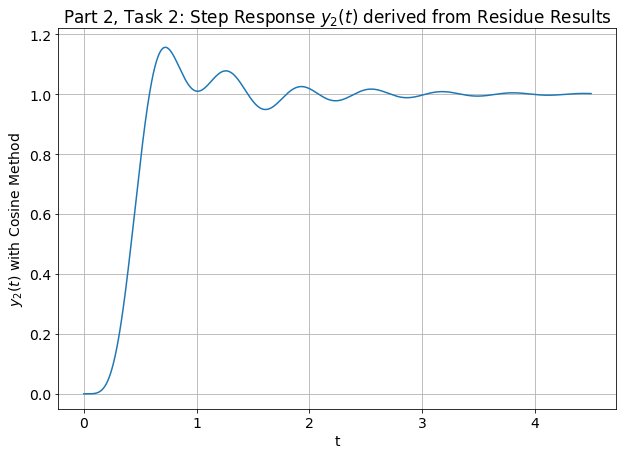
\includegraphics[scale = 0.6]{Lab 6 - Plots/Part2-Task2.png}\\[1.0 cm]
\end{center}

The plot below shows the step response of the high order differential found using the Python package command scipy.signal.step(). As stated before, this plot is visually identical to the plot found using the cosine method. The axes and peaks also match and have not been stretched or shifted. This provides credibility to both plots. 
\\

\begin{center}
	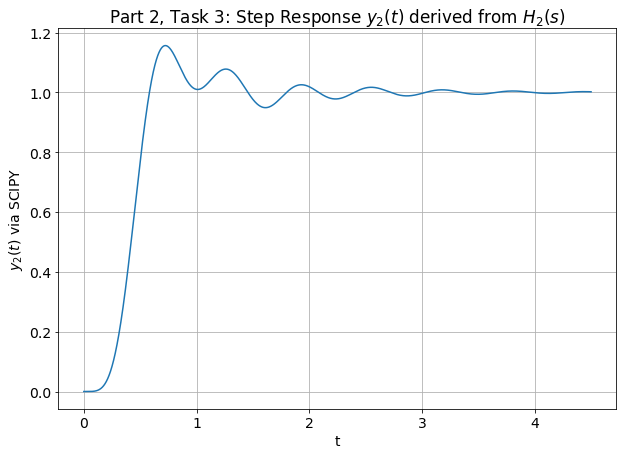
\includegraphics[scale = 0.6]{Lab 6 - Plots/Part2-Task3.png}\\[1.0 cm]
\end{center}

\section{Error Analysis}

The main problem I had in this lab was with my index of iteration for the cosine method step response function. I originally used the function range(0, 5) to try to match the number of loop entries to the number of array elements. This failed to include some values such that the plot produced did not match the subsequent Python result. At the TA's recommendation, I fixed this problem by changing the parameter of the function to range(len(R)) which allowed Python to obtain the proper size. \\

I also initially failed to remove the multiplication by two in the same function implementation for the cosine method from Equation 1. By reviewing the lab manual's instructions, I came to understand that it was already accounted for in the residue results. I fixed the incorrect plot by removing this unnecessary number. \\
	
\section{Questions}

1. A non-complex pole or residue term has no imaginary part and consequently no phase. Looking at the cosine method in Equation 1, we see that both the imaginary part of the pole and the phase of the residue are within the cosine funcion. Thus, the $ \omega t $ term will go to zero and be added with a phase of zero. The result will be a $ cos(0) $ which is just one. The solution becomes simply an exponential term with the step function, which is what we would expect from the regular non-complex method. \\

2. The lab expectations, instructions, and deliverables were communicated clearly. \\
	
\section{Conclusion}

This lab developed our understanding of partial fraction expansion, introducing the method in Python using scipy.signal.residue(). It taught us the three parts to the expansion we can expect to be returned. It allowed for practice with the cosine method, and also grew our familiarity with implementing functions as numerator and denominator arrays. We continued improving in our ability to use scipy.signal.step() to find the step response of an input. \\

If this lab were repeated, I would introduce an example where the K coefficient array returned by the residue function has an actual value. Without this parameter filled in, it can be hard to grasp what it represents. Through this lab, I was reminded of the need to always consider what the problem is we are trying to solve, and what the requested solution is. This was specifically necessary to set the numerator and denominator arrays with the proper values. Taking a little extra time upfront to consider a problem will continue to be invaluable going forward. \\
	
\newpage
\appendix
\section*{Appendix - Print Output}

Part 1, Task 3:
\begin{center}
	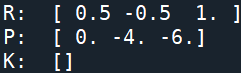
\includegraphics[scale = 1.25]{Lab 6 - Print Outputs/Part1-Task3.png}\\[1.0 cm]
\end{center}

Part 2, Task 1:
\begin{center}
	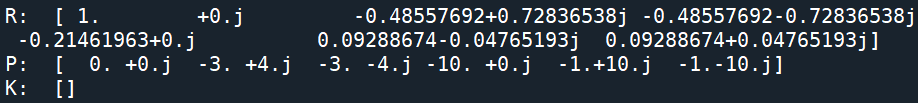
\includegraphics[scale = 0.92]{Lab 6 - Print Outputs/Part2-Task1.png}\\[1.0 cm]
\end{center}

\newpage
\begin{thebibliography}{111}
		
	\bibitem{S}
	Sullivan, Dennis M. (2018) {\it  Signals and Systems for Electrical Engineers I}. Nevada: CreateSpace Independent Publishing Platform.
		
\end{thebibliography}
\end{document}

% Lab Report based on template created by Roza Aceska.